% Options for packages loaded elsewhere
\PassOptionsToPackage{unicode}{hyperref}
\PassOptionsToPackage{hyphens}{url}
\documentclass[
  spanish,
]{article}
\usepackage{xcolor}
\usepackage[margin=1in]{geometry}
\usepackage{amsmath,amssymb}
\setcounter{secnumdepth}{5}
\usepackage{iftex}
\ifPDFTeX
  \usepackage[T1]{fontenc}
  \usepackage[utf8]{inputenc}
  \usepackage{textcomp} % provide euro and other symbols
\else % if luatex or xetex
  \usepackage{unicode-math} % this also loads fontspec
  \defaultfontfeatures{Scale=MatchLowercase}
  \defaultfontfeatures[\rmfamily]{Ligatures=TeX,Scale=1}
\fi
\usepackage{lmodern}
\ifPDFTeX\else
  % xetex/luatex font selection
\fi
% Use upquote if available, for straight quotes in verbatim environments
\IfFileExists{upquote.sty}{\usepackage{upquote}}{}
\IfFileExists{microtype.sty}{% use microtype if available
  \usepackage[]{microtype}
  \UseMicrotypeSet[protrusion]{basicmath} % disable protrusion for tt fonts
}{}
\makeatletter
\@ifundefined{KOMAClassName}{% if non-KOMA class
  \IfFileExists{parskip.sty}{%
    \usepackage{parskip}
  }{% else
    \setlength{\parindent}{0pt}
    \setlength{\parskip}{6pt plus 2pt minus 1pt}}
}{% if KOMA class
  \KOMAoptions{parskip=half}}
\makeatother
\usepackage{graphicx}
\makeatletter
\newsavebox\pandoc@box
\newcommand*\pandocbounded[1]{% scales image to fit in text height/width
  \sbox\pandoc@box{#1}%
  \Gscale@div\@tempa{\textheight}{\dimexpr\ht\pandoc@box+\dp\pandoc@box\relax}%
  \Gscale@div\@tempb{\linewidth}{\wd\pandoc@box}%
  \ifdim\@tempb\p@<\@tempa\p@\let\@tempa\@tempb\fi% select the smaller of both
  \ifdim\@tempa\p@<\p@\scalebox{\@tempa}{\usebox\pandoc@box}%
  \else\usebox{\pandoc@box}%
  \fi%
}
% Set default figure placement to htbp
\def\fps@figure{htbp}
\makeatother
\ifLuaTeX
\usepackage[bidi=basic]{babel}
\else
\usepackage[bidi=default]{babel}
\fi
% get rid of language-specific shorthands (see #6817):
\let\LanguageShortHands\languageshorthands
\def\languageshorthands#1{}
\setlength{\emergencystretch}{3em} % prevent overfull lines
\providecommand{\tightlist}{%
  \setlength{\itemsep}{0pt}\setlength{\parskip}{0pt}}
\usepackage{booktabs}
\usepackage{longtable}
\usepackage{array}
\usepackage{multirow}
\usepackage{float}
\usepackage{colortbl}
\usepackage{xcolor}
\usepackage{pdflscape}
\usepackage{geometry}
\geometry{margin=2.5cm}
\usepackage{fancyhdr}
\pagestyle{fancy}
\fancyhead[L]{\small Contraste de Hipótesis}
\fancyhead[R]{\small Tesis --- Experiencia Gastronómica}
\fancyfoot[C]{\thepage}
\renewcommand{\headrulewidth}{0.4pt}
\usepackage{caption}
\captionsetup{font=small, labelfont=bf}
\usepackage{booktabs}
\usepackage{longtable}
\usepackage{array}
\usepackage{multirow}
\usepackage{wrapfig}
\usepackage{float}
\usepackage{colortbl}
\usepackage{pdflscape}
\usepackage{tabu}
\usepackage{threeparttable}
\usepackage{threeparttablex}
\usepackage[normalem]{ulem}
\usepackage{makecell}
\usepackage{xcolor}
\usepackage{bookmark}
\IfFileExists{xurl.sty}{\usepackage{xurl}}{} % add URL line breaks if available
\urlstyle{same}
\hypersetup{
  pdftitle={Contraste de Hipótesis},
  pdfauthor={Ariana-Fernanda Valeria Vidal Tapia},
  pdflang={es},
  hidelinks,
  pdfcreator={LaTeX via pandoc}}

\title{Contraste de Hipótesis}
\usepackage{etoolbox}
\makeatletter
\providecommand{\subtitle}[1]{% add subtitle to \maketitle
  \apptocmd{\@title}{\par {\large #1 \par}}{}{}
}
\makeatother
\subtitle{Impacto de los factores de la experiencia gastronómica en la
toma de decisiones del comensal}
\author{Ariana-Fernanda Valeria Vidal Tapia}
\date{16 de April de 2026}

\begin{document}
\maketitle

{
\setcounter{tocdepth}{3}
\tableofcontents
}
\section{Carga de datos y
librerías}\label{carga-de-datos-y-libreruxedas}

Este informe toma como insumo la tabla de decisión del informe anterior
(verificación de supuestos). Para cada variable dependiente se aplica la
prueba más adecuada según el cumplimiento de normalidad y
homocedasticidad. Adicionalmente, dado que los datos son escalas Likert
(ordinales), se ejecuta sistemáticamente el enfoque no paramétrico como
análisis principal y el paramétrico como análisis de sensibilidad.

\newpage

\section{Hipótesis general}\label{hipuxf3tesis-general}

\begin{quote}
\textbf{\(H_0\):} La variación en los elementos de la experiencia
gastronómica NO influye significativamente en la toma de decisiones del
comensal.

\textbf{\(H_1\):} La variación en los elementos de la experiencia
gastronómica influye significativamente en la toma de decisiones del
comensal.
\end{quote}

Se evalúa comparando las cuatro condiciones experimentales (base,
servicio degradado, producto degradado, entorno degradado) sobre las
tres variables dependientes: satisfacción (I1), intención de revisitar
(I2) e intención de recomendar (I3).

\subsection{Prueba ómnibus:
Kruskal-Wallis}\label{prueba-uxf3mnibus-kruskal-wallis}

\begin{table}[!h]
\centering
\begin{tabular}{lcccc>{}c}
\toprule
Variable & $H$ & $gl$ & $p$ & $\eta^2_H$ & Significativo\\
\midrule
Satisfacción (I1) & 50.298 & 3 & < .001 & 0.275 & \textcolor{teal}{Sí}\\
Revisitar (I2) & 64.132 & 3 & < .001 & 0.355 & \textcolor{teal}{Sí}\\
\bottomrule
\end{tabular}
\end{table}

\textbf{Interpretación de \(\eta^2_H\):} valores de 0.01, 0.06 y 0.14 se
consideran efectos pequeño, mediano y grande, respectivamente.

\subsection{Prueba para I3 (recomendar):
Chi-cuadrado}\label{prueba-para-i3-recomendar-chi-cuadrado}

Al ser I3 una variable binaria (Sí/No), se utiliza la prueba de
chi-cuadrado de independencia para evaluar si la proporción de
comensales que recomendarían difiere entre condiciones.

\begin{table}[!h]
\centering
\caption{\label{tab:chi-tabla-print}Tabla de contingencia: Condición vs. Recomendaría}
\centering
\begin{tabular}[t]{lcc}
\toprule
Condición & No recomendaría & Sí recomendaría\\
\midrule
Base (todo bien) & 2 (4.5\%) & 42 (95.5\%)\\
Servicio degradado & 23 (52.3\%) & 21 (47.7\%)\\
Producto degradado & 31 (70.5\%) & 13 (29.5\%)\\
Entorno degradado & 31 (70.5\%) & 13 (29.5\%)\\
\bottomrule
\end{tabular}
\end{table}

\begin{table}[!h]
\centering
\begin{tabular}{lc}
\toprule
Estadístico & Valor\\
\midrule
$\chi^2$ & 51.166\\
$gl$ & 3\\
$p$ & < .001\\
$V$ de Cramér & 0.539\\
\bottomrule
\end{tabular}
\end{table}

\textbf{Interpretación de la \(V\) de Cramér:} valores de 0.10, 0.30 y
0.50 se interpretan como efectos pequeño, mediano y grande,
respectivamente.

\subsection{Análisis de sensibilidad: ANOVA de
Welch}\label{anuxe1lisis-de-sensibilidad-anova-de-welch}

Como análisis complementario, se ejecuta el ANOVA de Welch (robusto ante
varianzas desiguales) para I1 e I2.

\begin{table}[!h]
\centering
\begin{tabular}{lccccc}
\toprule
Variable & $F$ & $gl_1$ & $gl_2$ & $p$ & Significativo\\
\midrule
Satisfacción (I1) & 36.438 & 3 & 89.5 & < .001 & Sí\\
Revisitar (I2) & 42.373 & 3 & 94.3 & < .001 & Sí\\
\bottomrule
\end{tabular}
\end{table}

La convergencia de resultados entre Kruskal-Wallis y Welch ANOVA
fortalece la robustez de las conclusiones.

\newpage

\section{Hipótesis específicas: Comparaciones
focalizadas}\label{hipuxf3tesis-especuxedficas-comparaciones-focalizadas}

Cada hipótesis específica se contrasta comparando la condición degradada
correspondiente contra la línea base (Semana 1).

\subsection{Comparaciones post-hoc: Test de
Dunn}\label{comparaciones-post-hoc-test-de-dunn}

Se aplica el test de Dunn con corrección de Bonferroni. El interés
principal está en los tres contrastes contra la base, aunque se reportan
todas las comparaciones.

\begin{table}[!h]
\centering\begingroup\fontsize{9}{11}\selectfont

\begin{tabular}{llccc}
\toprule
Variable & Comparación & $Z$ & $p$ ajustado & Significativo\\
\midrule
\addlinespace[0.3em]
\multicolumn{5}{l}{\textbf{Revisitar (I2)}}\\
\hspace{1em}Satisfacción (I1) & Base (todo bien) - Entorno degradado & 6.288 & < .001 & Sí\\
\hspace{1em}Satisfacción (I1) & Base (todo bien) - Producto degradado & 5.975 & < .001 & Sí\\
\hspace{1em}Satisfacción (I1) & Entorno degradado - Producto degradado & -0.313 & 1.0000 & No\\
\hspace{1em}Satisfacción (I1) & Base (todo bien) - Servicio degradado & 4.314 & < .001 & Sí\\
\hspace{1em}Satisfacción (I1) & Entorno degradado - Servicio degradado & -1.973 & 0.1454 & No\\
\hspace{1em}Satisfacción (I1) & Producto degradado - Servicio degradado & -1.660 & 0.2905 & No\\
\addlinespace[0.3em]
\multicolumn{5}{l}{\textbf{Satisfacción (I1)}}\\
\hspace{1em}Revisitar (I2) & Base (todo bien) - Entorno degradado & 7.024 & < .001 & Sí\\
\hspace{1em}Revisitar (I2) & Base (todo bien) - Producto degradado & 6.812 & < .001 & Sí\\
\hspace{1em}Revisitar (I2) & Entorno degradado - Producto degradado & -0.212 & 1.0000 & No\\
\hspace{1em}Revisitar (I2) & Base (todo bien) - Servicio degradado & 5.040 & < .001 & Sí\\
\hspace{1em}Revisitar (I2) & Entorno degradado - Servicio degradado & -1.984 & 0.1418 & No\\
\hspace{1em}Revisitar (I2) & Producto degradado - Servicio degradado & -1.772 & 0.2293 & No\\
\bottomrule
\end{tabular}
\endgroup{}
\end{table}

\subsection{\texorpdfstring{Tamaño del efecto por pares: \(r\) de
rango}{Tamaño del efecto por pares: r de rango}}\label{tamauxf1o-del-efecto-por-pares-r-de-rango}

Para cada comparación significativa se calcula el tamaño del efecto
\(r = \frac{Z}{\sqrt{n_1 + n_2}}\), donde \(n_1\) y \(n_2\) son los
tamaños de los grupos comparados.

\begin{table}[!h]
\centering\begingroup\fontsize{9}{11}\selectfont

\begin{tabular}{llcccc}
\toprule
Variable & Comparación & $Z$ & $p$ ajustado & $r$ & Magnitud\\
\midrule
\addlinespace[0.3em]
\multicolumn{6}{l}{\textbf{Revisitar (I2)}}\\
\hspace{1em}Satisfacción (I1) & Base (todo bien) - Entorno degradado & 6.288 & < .001 & 0.670 & Grande\\
\hspace{1em}Satisfacción (I1) & Base (todo bien) - Producto degradado & 5.975 & < .001 & 0.637 & Grande\\
\hspace{1em}Satisfacción (I1) & Entorno degradado - Producto degradado & -0.313 & 1.0000 & 0.033 & Trivial\\
\hspace{1em}Satisfacción (I1) & Base (todo bien) - Servicio degradado & 4.314 & < .001 & 0.460 & Mediano\\
\hspace{1em}Satisfacción (I1) & Entorno degradado - Servicio degradado & -1.973 & 0.1454 & 0.210 & Pequeño\\
\hspace{1em}Satisfacción (I1) & Producto degradado - Servicio degradado & -1.660 & 0.2905 & 0.177 & Pequeño\\
\addlinespace[0.3em]
\multicolumn{6}{l}{\textbf{Satisfacción (I1)}}\\
\hspace{1em}Revisitar (I2) & Base (todo bien) - Entorno degradado & 7.024 & < .001 & 0.749 & Grande\\
\hspace{1em}Revisitar (I2) & Base (todo bien) - Producto degradado & 6.812 & < .001 & 0.726 & Grande\\
\hspace{1em}Revisitar (I2) & Entorno degradado - Producto degradado & -0.212 & 1.0000 & 0.023 & Trivial\\
\hspace{1em}Revisitar (I2) & Base (todo bien) - Servicio degradado & 5.040 & < .001 & 0.537 & Grande\\
\hspace{1em}Revisitar (I2) & Entorno degradado - Servicio degradado & -1.984 & 0.1418 & 0.211 & Pequeño\\
\hspace{1em}Revisitar (I2) & Producto degradado - Servicio degradado & -1.772 & 0.2293 & 0.189 & Pequeño\\
\bottomrule
\end{tabular}
\endgroup{}
\end{table}

\textbf{Interpretación de \(r\):} valores de 0.10, 0.30 y 0.50
corresponden a efectos pequeño, mediano y grande (Cohen, 1988).

\subsection{Comparaciones por pares para I3: Test exacto de
Fisher}\label{comparaciones-por-pares-para-i3-test-exacto-de-fisher}

Para la variable binaria I3 (recomendar), se comparan las proporciones
de cada condición degradada contra la base usando el test exacto de
Fisher con corrección de Bonferroni.

\begin{table}[!h]
\centering
\begin{tabular}{lccccc}
\toprule
Comparación & \% Base & \% Degradada & $OR$ & $p$ & Sig. (Bonf.)\\
\midrule
Base vs. Servicio degradado & 95.5\% & 47.7\% & 0.05 & < .001 & Sí\\
Base vs. Producto degradado & 95.5\% & 29.5\% & 0.02 & < .001 & Sí\\
Base vs. Entorno degradado & 95.5\% & 29.5\% & 0.02 & < .001 & Sí\\
\bottomrule
\end{tabular}
\end{table}

Se aplica corrección de Bonferroni dividiendo \(\alpha = 0.05\) entre 3
comparaciones (\(\alpha_{corregido} = 0.0167\)). El Odds Ratio (\(OR\))
indica cuántas veces más probable es recomendar en la condición base
respecto a la degradada.

\newpage

\section{Verificación de la manipulación
experimental}\label{verificaciuxf3n-de-la-manipulaciuxf3n-experimental}

Se verifica formalmente que en cada condición degradada, la dimensión
manipulada fue percibida como significativamente peor que en la línea
base, y que las dimensiones no manipuladas se mantuvieron estables.

\begin{table}[!h]
\centering\begingroup\fontsize{9}{11}\selectfont

\resizebox{\ifdim\width>\linewidth\linewidth\else\width\fi}{!}{
\begin{tabular}{llccccc}
\toprule
Dimensión & Condición & $M$ Base & $M$ Degradada & Diferencia & $p$ (Mann-Whitney) & Expectativa\\
\midrule
Producto & Servicio degradado & 3.77 & 3.44 & -0.33 & 0.0155 & Debe mantenerse\\
Producto & Producto degradado & 3.77 & 2.72 & -1.05 & < .001 & Debe bajar\\
Producto & Entorno degradado & 3.77 & 3.15 & -0.61 & < .001 & Debe mantenerse\\
Servicio & Servicio degradado & 4.30 & 3.11 & -1.20 & < .001 & Debe bajar\\
Servicio & Producto degradado & 4.30 & 4.33 & 0.02 & 0.7042 & Debe mantenerse\\
\addlinespace
Servicio & Entorno degradado & 4.30 & 3.95 & -0.36 & 0.0443 & Debe mantenerse\\
Entorno & Servicio degradado & 4.33 & 4.11 & -0.22 & 0.0419 & Debe mantenerse\\
Entorno & Producto degradado & 4.33 & 4.16 & -0.16 & 0.0713 & Debe mantenerse\\
Entorno & Entorno degradado & 4.33 & 2.29 & -2.03 & < .001 & Debe bajar\\
\bottomrule
\end{tabular}}
\endgroup{}
\end{table}

Las celdas donde la expectativa es ``Debe bajar'' deberían mostrar
diferencias negativas significativas. Las celdas con ``Debe mantenerse''
deberían mostrar diferencias no significativas o muy pequeñas.

\newpage

\section{Análisis de regresión: Factor más influyente (Objetivo
4)}\label{anuxe1lisis-de-regresiuxf3n-factor-muxe1s-influyente-objetivo-4}

Para identificar cuál de las tres dimensiones (producto, servicio,
entorno) tiene mayor peso relativo sobre las variables dependientes, se
ajustan modelos de regresión con los datos combinados de las 4 semanas
(\(n = 176\)).

\subsection{Regresión lineal múltiple (Satisfacción e Intención de
revisitar)}\label{regresiuxf3n-lineal-muxfaltiple-satisfacciuxf3n-e-intenciuxf3n-de-revisitar}

\subsubsection{Modelo para Satisfacción
(I1)}\label{modelo-para-satisfacciuxf3n-i1}

\begin{table}[!h]
\centering
\caption{\label{tab:reg-satisf-print}Modelo Satisfacción: $R^2$ = 0.467, $R^2_{aj}$ = 0.458, $F$(3, 172) = 50.21}
\centering
\begin{tabular}[t]{lccccc}
\toprule
Predictor & $b$ & $EE$ & $t$ & $p$ & $\beta$\\
\midrule
Intercepto & -0.4648 & 0.3280 & -1.4170 & 0.1583 & NA\\
Producto & 0.6219 & 0.0687 & 9.0579 & < .001 & 0.521\\
Servicio & 0.2052 & 0.0594 & 3.4577 & < .001 & 0.197\\
Entorno & 0.2342 & 0.0562 & 4.1639 & < .001 & 0.238\\
\bottomrule
\end{tabular}
\end{table}

\subsubsection{Modelo para Revisitar
(I2)}\label{modelo-para-revisitar-i2}

\begin{table}[!h]
\centering
\caption{\label{tab:reg-revis-print}Modelo Revisitar: $R^2$ = 0.463, $R^2_{aj}$ = 0.453, $F$(3, 172) = 49.35}
\centering
\begin{tabular}[t]{lccccc}
\toprule
Predictor & $b$ & $EE$ & $t$ & $p$ & $\beta$\\
\midrule
Intercepto & -0.7827 & 0.3489 & -2.2434 & 0.0261 & NA\\
Producto & 0.6224 & 0.0730 & 8.5230 & < .001 & 0.509\\
Servicio & 0.1472 & 0.0631 & 2.3322 & 0.0208 & 0.138\\
Entorno & 0.3359 & 0.0598 & 5.6149 & < .001 & 0.333\\
\bottomrule
\end{tabular}
\end{table}

El coeficiente estandarizado (\(\beta\)) permite comparar directamente
la importancia relativa de cada dimensión. El predictor con mayor
\(|\beta|\) es el factor más influyente.

\subsection{Regresión logística
(Recomendar)}\label{regresiuxf3n-loguxedstica-recomendar}

\begin{table}[!h]
\centering
\caption{\label{tab:reg-logist-print}Regresión logística --- Recomendar. AIC = 181.1}
\centering
\begin{tabular}[t]{lccccc}
\toprule
Predictor & $b$ & $EE$ & $z$ & $p$ & $OR$\\
\midrule
Intercepto & -9.7057 & 1.6289 & -5.9586 & < .001 & 0.000\\
Producto & 1.6984 & 0.3083 & 5.5097 & < .001 & 5.465\\
Servicio & 0.4211 & 0.2093 & 2.0117 & 0.0442 & 1.524\\
Entorno & 0.6746 & 0.2139 & 3.1542 & 0.0016 & 1.963\\
\bottomrule
\end{tabular}
\end{table}

El Odds Ratio (\(OR\)) indica el cambio multiplicativo en la
probabilidad de recomendar por cada unidad de aumento en el predictor,
manteniendo los demás constantes. Un \(OR > 1\) indica efecto positivo.

\subsection{Comparación de la importancia
relativa}\label{comparaciuxf3n-de-la-importancia-relativa}

\begin{figure}[H]

{\centering 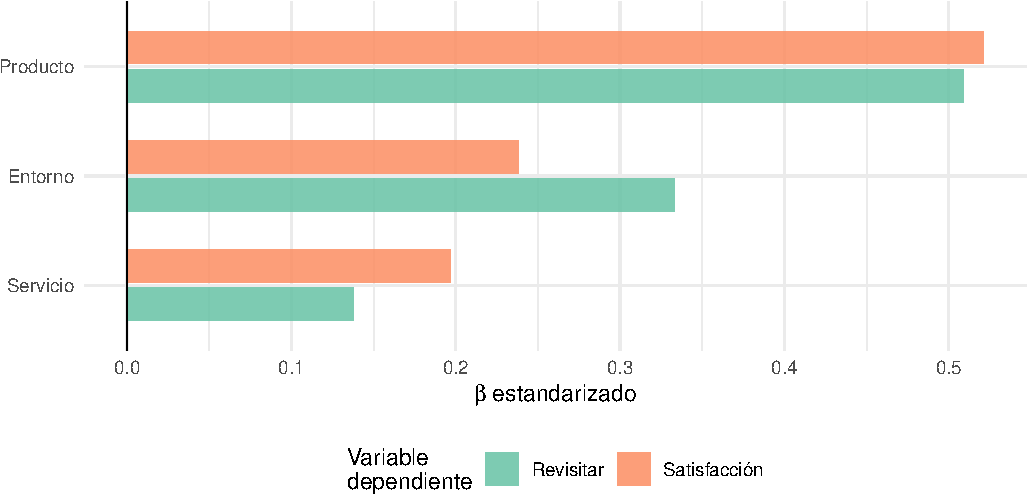
\includegraphics[width=0.95\linewidth]{02_contraste_hipotesis_files/figure-latex/comparar-betas-1} 

}

\caption{Coeficientes estandarizados ($\beta$) de cada dimensión sobre Satisfacción y Revisitar.}\label{fig:comparar-betas}
\end{figure}

\newpage

\section{Matriz de correlaciones de Spearman (Objetivo
5)}\label{matriz-de-correlaciones-de-spearman-objetivo-5}

Para evaluar la relación entre la percepción sensorial de la experiencia
gastronómica y la toma de decisiones del comensal.

\begin{table}[!h]
\centering\begingroup\fontsize{9}{11}\selectfont

\begin{tabular}{lcccccc}
\toprule
  & Producto & Servicio & Entorno & Satisfacción & Revisitar & Recomendar\\
\midrule
Producto & --- & 0.220** & 0.227** & 0.612*** & 0.587*** & 0.534***\\
Servicio & 0.220** & --- & 0.190* & 0.333*** & 0.255*** & 0.257***\\
Entorno & 0.227** & 0.190* & --- & 0.380*** & 0.448*** & 0.339***\\
Satisfacción & 0.612*** & 0.333*** & 0.380*** & --- & 0.810*** & 0.674***\\
Revisitar & 0.587*** & 0.255*** & 0.448*** & 0.810*** & --- & 0.698***\\
\addlinespace
Recomendar & 0.534*** & 0.257*** & 0.339*** & 0.674*** & 0.698*** & ---\\
\bottomrule
\multicolumn{7}{l}{\rule{0pt}{1em}* p < .05, ** p < .01, *** p < .001 (Spearman).}\\
\end{tabular}
\endgroup{}
\end{table}

\newpage

\section{Resumen de resultados por
hipótesis}\label{resumen-de-resultados-por-hipuxf3tesis}

\begingroup\fontsize{9}{11}\selectfont

\begin{tabu} to \linewidth {>{\raggedright\arraybackslash}p{6cm}>{\raggedright\arraybackslash}p{10cm}}
\toprule
Hipótesis & Resultado\\
\midrule
General: La variación en los elementos de la experiencia gastronómica influye en la toma de decisiones del comensal. & Kruskal-Wallis significativo para Satisfacción y Revisitar; Chi-cuadrado significativo para Recomendar. Se acepta $H_1$.\\
Específica 1: La variación en la calidad del producto influye en la toma de decisiones. & Comparación Base vs. Producto degradado en Dunn y Fisher. Ver tabla de post-hoc.\\
Específica 2: La variación en la calidad del servicio afecta la toma de decisiones. & Comparación Base vs. Servicio degradado en Dunn y Fisher. Ver tabla de post-hoc.\\
Específica 3: La variación en el entorno influye en la toma de decisiones. & Comparación Base vs. Entorno degradado en Dunn y Fisher. Ver tabla de post-hoc.\\
Específica 4: Factor sensorial más influyente. & El predictor con mayor $|\beta|$ en la regresión es el más influyente. Ver gráfico de coeficientes.\\
\addlinespace
Específica 5: Relación entre percepción sensorial y toma de decisiones. & Correlaciones de Spearman significativas. Ver matriz de correlaciones.\\
\bottomrule
\end{tabu}
\endgroup{}

Los resultados detallados (estadísticos exactos, \(p\)-valores y tamaños
del efecto) se encuentran en las tablas correspondientes de cada sección
anterior.

\end{document}
